\chapter{模擬環境}
%\renewcommand{\baselinestretch}{10.0} %設定行距
\section{模擬模型}
 在模擬的模型上,延用了學長之前組建的實體3D列印機,並將其轉為虛擬模型後放入CoppeliaSim,進行組裝、配置後以simExtFIBR3D.dll擴充CoppeliaSim將其與GCodeInterpreter程式進行整合,用以達成使用GCode控制CoppeliaSim中的3D列印機進行模擬列印展示之功能。\\
\begin{figure}[hbt!]
\center
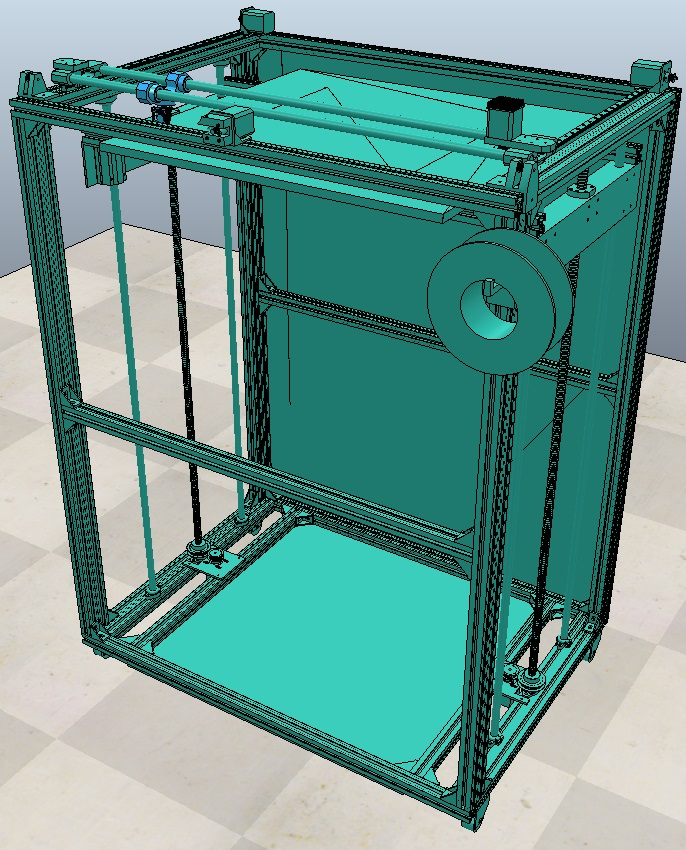
\includegraphics[width=13cm]{組合圖}
\caption{\Large 組合圖}
\label{組合圖}
\end{figure}

\newpage

\section{CoppeliaSim}
 CoppeliaSim是一套具有整合開發環境的機器人模擬軟體,基於分佈式控制體系架構,可以利用寫入嵌入式腳本、插件、ROS、BlueZero節點、RemoteAPI客戶端或自定義解決方案達成模型控制之效果。\\
\begin{figure}[hbt!]
\center

\includegraphics[width=10cm]{CoppeliaSim}
\caption{\Large CoppeliaSim Logo}
\end{figure}

並且在CoppeliaSim中,控制器可以用C / C ++、Python、Java、Lua、Matlab或Octave進行編寫。\\
\subsection{使用原因}
 本模擬之最終目標是希望可以在虛擬環境中進行3D列印的結果展示,通過虛擬環境中的模擬後,在每次修改零件並更新Gcode後可以直接展示列印的狀況,且在虛擬環境中不會有費用的支出,所以可以用於檢視所列印出之成果後,再進行圖檔修正或設計修改,除此之外CoppeliaSim的虛擬環境更接近真實環境,基於以上原因,所以此專題選擇CoppeliaSim做為模擬的環境。\\
\subsection{RemoteAPI}
 RemoteAPI(Remote Application Programming Interface)是CoppeliaSim API框架的一部分。它允許CoppeliaSim與外部應用程序之間的通訊,是跨平台並支持服務調用和雙向數據流。有兩個不同的版本/框架分別為:Remote API 和The B0-based remote API。\\
\subsection{功能列}
\begin{enumerate}
\item 以下為簡易功能說明:
\begin{figure}[hbt!]
\center
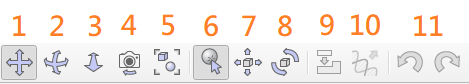
\includegraphics[width=11cm]{toolBar}
\caption{\Large CoppeliaSim 工具列}
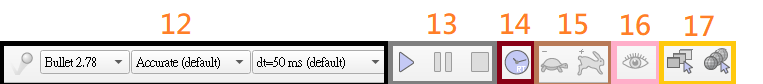
\includegraphics[width=13cm]{toolBar2}
\caption{\Large CoppeliaSim 工具列(續)}
\end{figure}
\begin{table}[hbt!]
\center
\large
\setlength{\tabcolsep}{0.75cm}{
\begin{tabular}{|c|c|c|c|}
\hline  代號 & 功能說明 & 代號 & 功能說明\\
\hline  1 &畫面平移& 10 &複製所有設定\\
\hline  2 &畫面旋轉& 11 &回復/取消回復\\
\hline  3 &畫面縮放&12&模擬設定\\
\hline  4 &畫面視角&13&開始/暫停/停止 模擬\\
\hline  5 &畫面縮放至適當大小&14&即時模擬切換\\
\hline  6 &選取物件&15&模擬速度控制\\
\hline  7 &移動物件&16&線程渲染/視覺化\\
\hline  8 &旋轉物件&17&場景/頁面 選擇\\
\hline  9 &加入/移出 樹狀結構&&\\
\hline
\end{tabular}}
\caption{\Large 功能說明}
\end{table}
\newpage
%\item 模擬執行\\%
\end{enumerate}
\section{FIBR3DEmul}
 FIBR3DEmul--是一個適用於3軸或3軸以上的FDM(熔融沉積成型)列印機,進行虛擬列印的開源軟體,在它之中包含了GCodeInterpreter(GCode解析器)、使用CMake生成的simExtFIBR3D.dll\\
\subsection{GCodeInterpreter}
\begin{figure}[hbt!]
\begin{center}
\includegraphics[width=8cm]{Gcode}
\caption{\Large GCodeInterpreter 介面功能介紹}\label{GCode}
\end{center}
\end{figure}
\newpage


\chapter{3D列印模擬流程}
\section{使用Inventor繪製uArm零件}
 模擬的第一步是先將更改後的uArm零件使用Inventor繪製出來後,再將其轉為Cura程式可接受的STL檔案格式。\\
\begin{figure}[hbt!]
\begin{center}
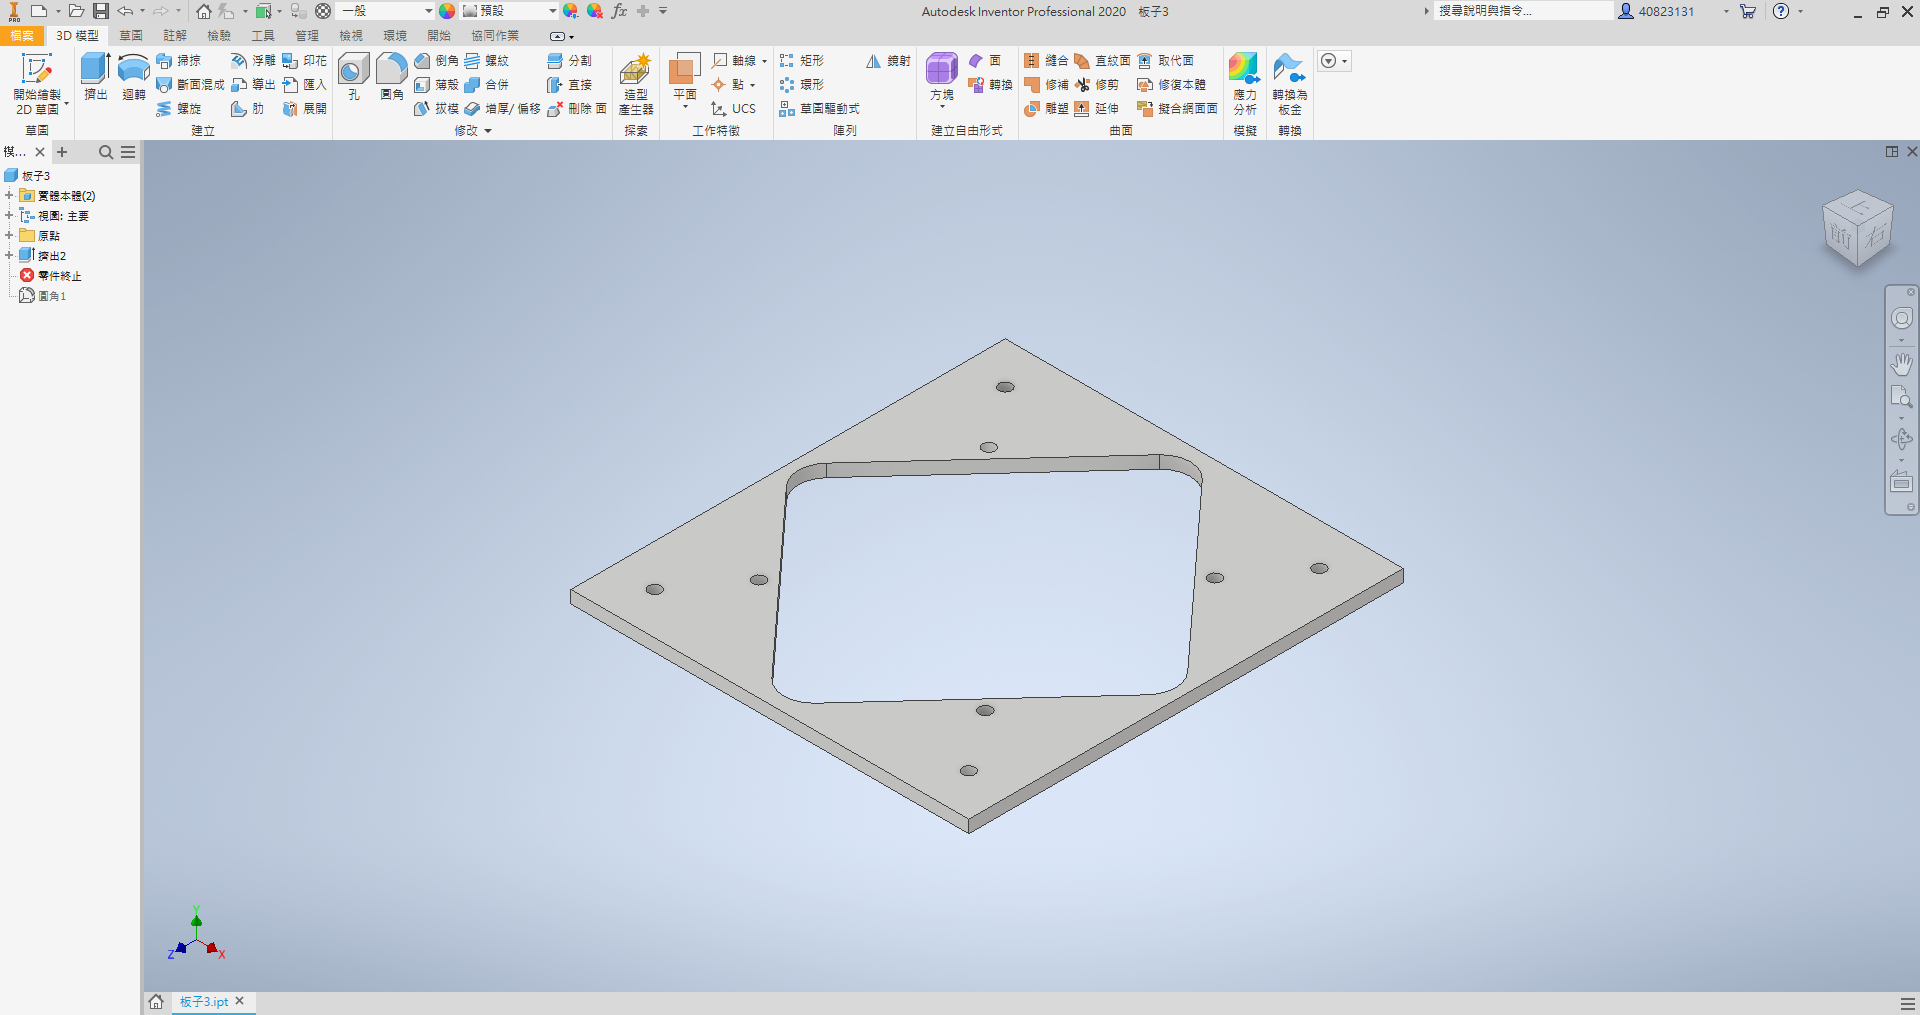
\includegraphics[width=8cm]{Inventor}
\caption{\Large 使用Inventor繪製零件}\label{Inventor}
\end{center}
\end{figure}
\section{使用Cura轉出G-Code檔}
 第二步將把上一步轉出的STL檔案轉入Cura程式中,可將零件們進行排列或旋轉方向放置到最佳的列印位置,進行切片後,轉出所需的G-Code檔案。\\
\begin{figure}[hbt!]
\begin{center}
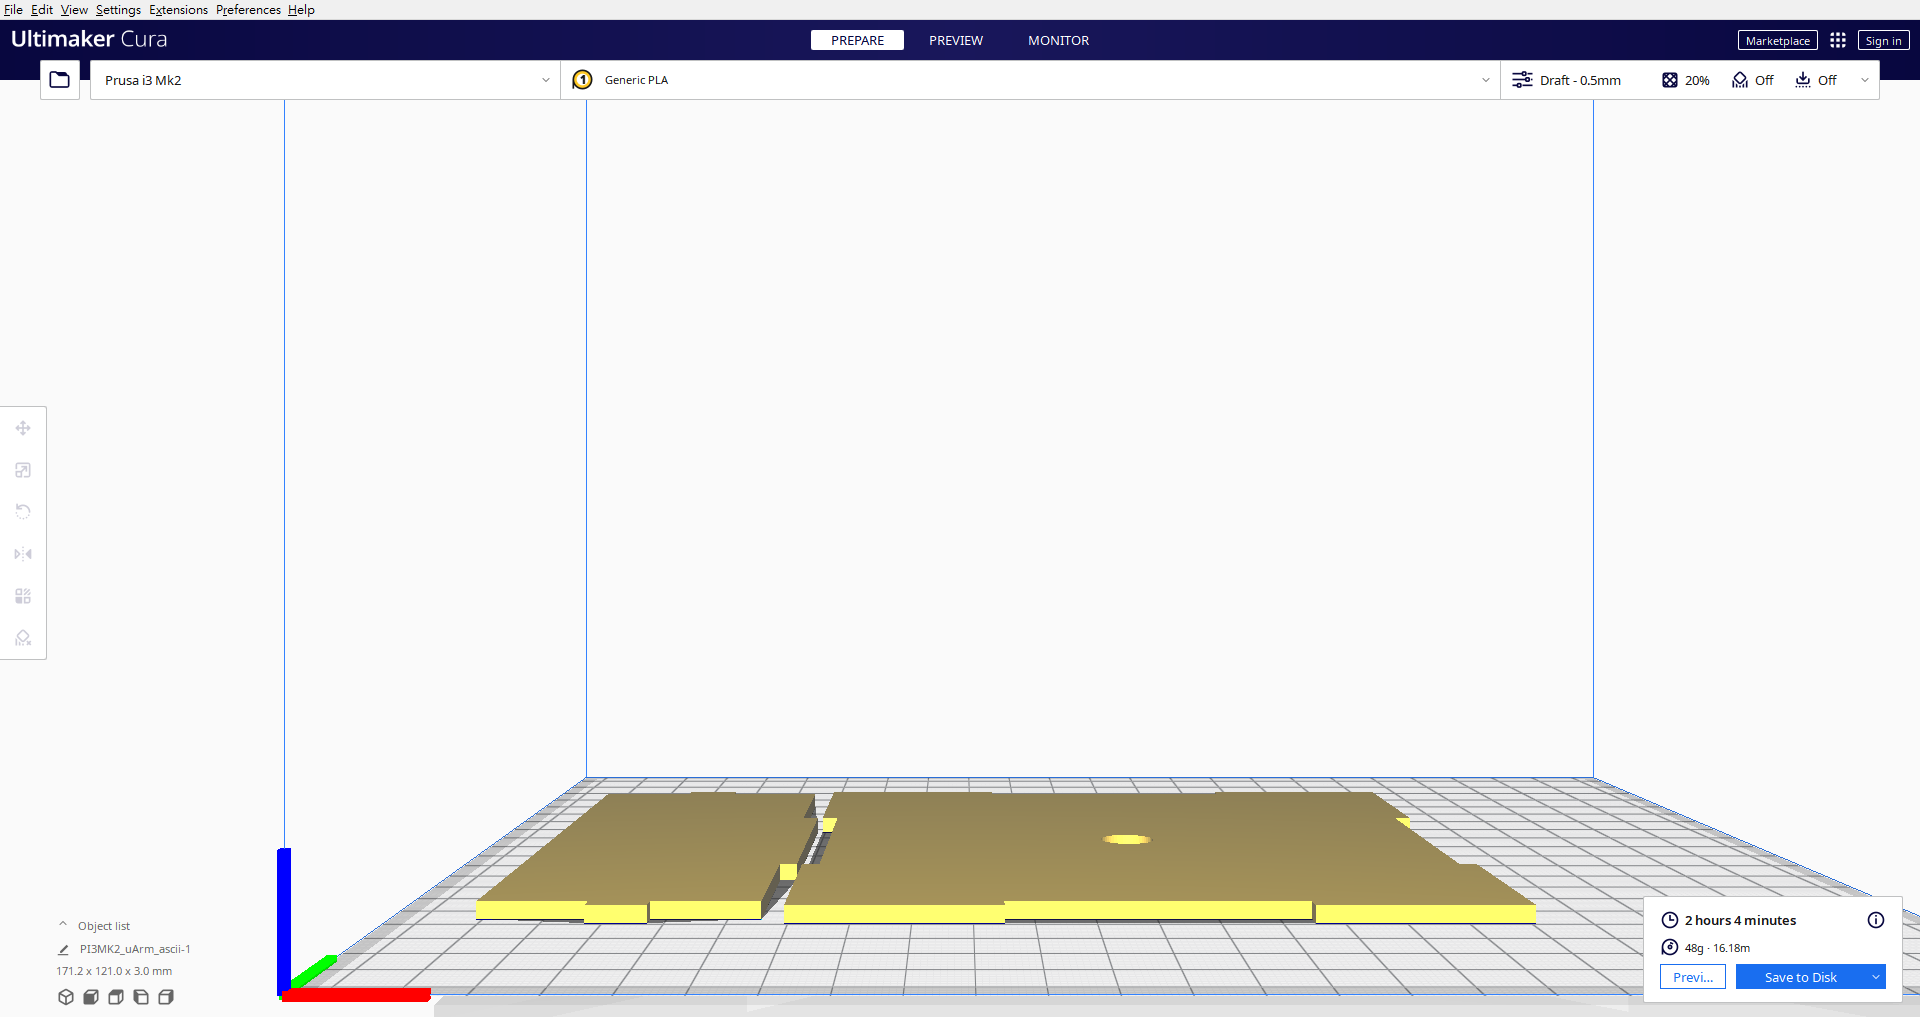
\includegraphics[width=8cm]{Cura}
\caption{\Large 用於轉出 G-Ccode 檔的切片軟體 Cura}\label{Cura}
\end{center}
\end{figure}
\section{更改G-Code檔}
 由於此列印模組之Z軸與本專題之3D列印機恰好相反,因此需修改有關的Z軸代碼後的數值為負值,還有一處需要修改,那就是擠出率的代碼,列印模組中擠出率代碼為A,但從Cura中轉出的G-Code中擠出率代碼為E,所以需將G-Code中的代碼E更改為A。
\begin{figure}[hbt!]
\begin{center}
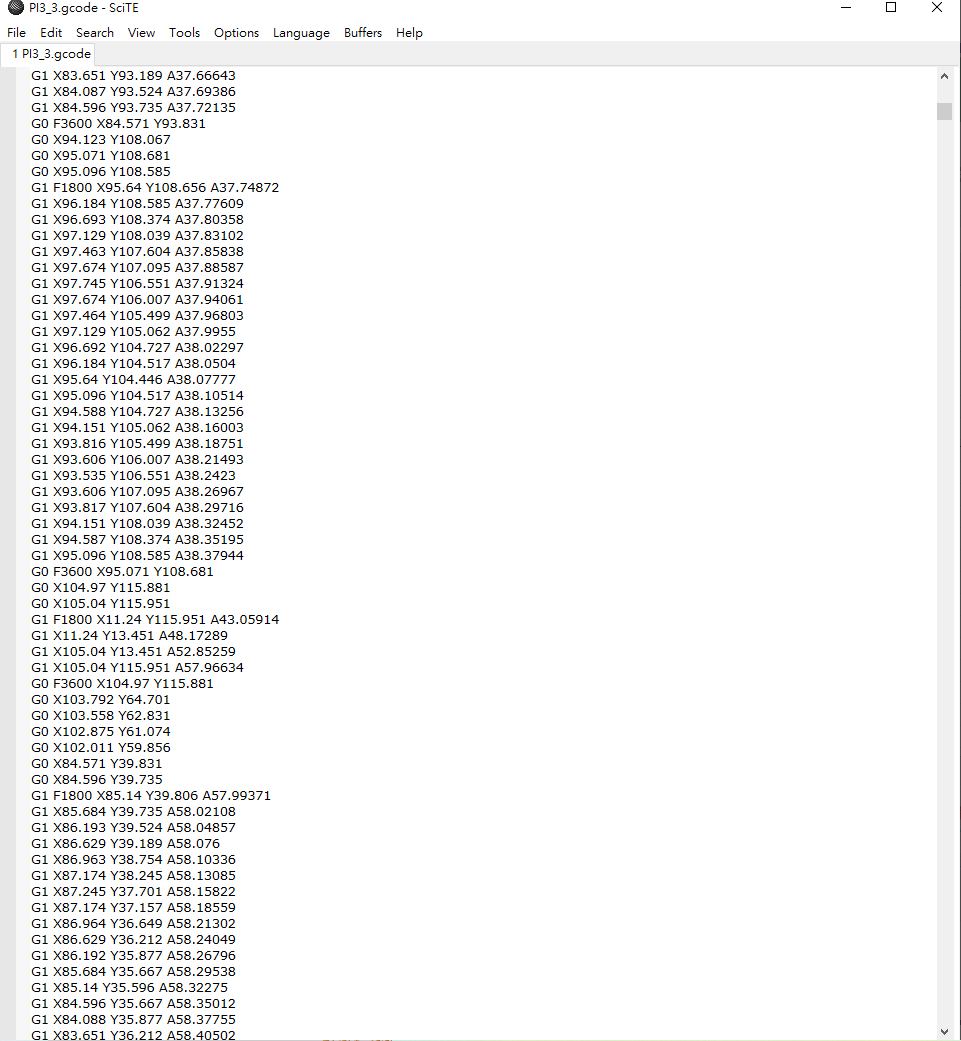
\includegraphics[width=8cm]{修改GCODE}
\caption{\Large 修改G-Code部分代碼}\label{修改GCODE}
\end{center}
\end{figure}
\section{將G-Code轉入GCodeInterpreter}
 第四步將修改好的G-Code檔案轉入GCodeInterpreter,按下連接鍵與CoppeliaSim連接後,進行模擬。\\
\begin{figure}[hbt!]
\begin{center}
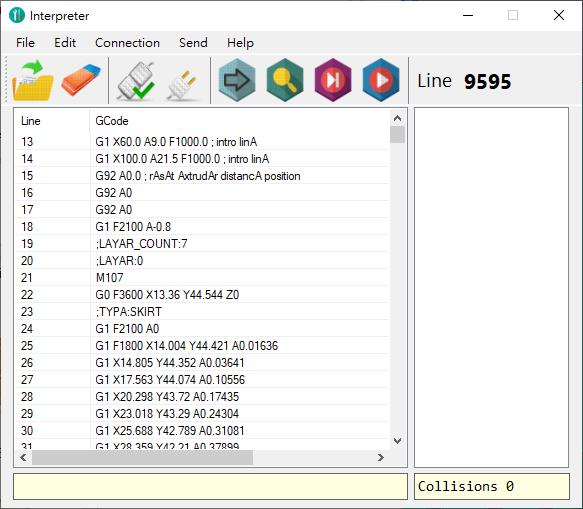
\includegraphics[width=8cm]{GCodeInterpreter}
\caption{\Large 模擬中的GCodeInterpreter畫面}\label{GCodeInterpreter}
\end{center}
\end{figure}
\section{uArm零件模擬列印結果}
 在CoppeliaSim模擬設定視窗中可以調整擠出材料的大小以及形狀(圓球或方塊),與GCodeInterpreter連接後,當GCodeInterpreter按下運行鍵後,開始列印模擬,在CoppeliaSim中也可以進行模擬列印整體速度調整,更加省時,下圖為模擬結果。\\
\begin{figure}[hbt!]
\begin{center}
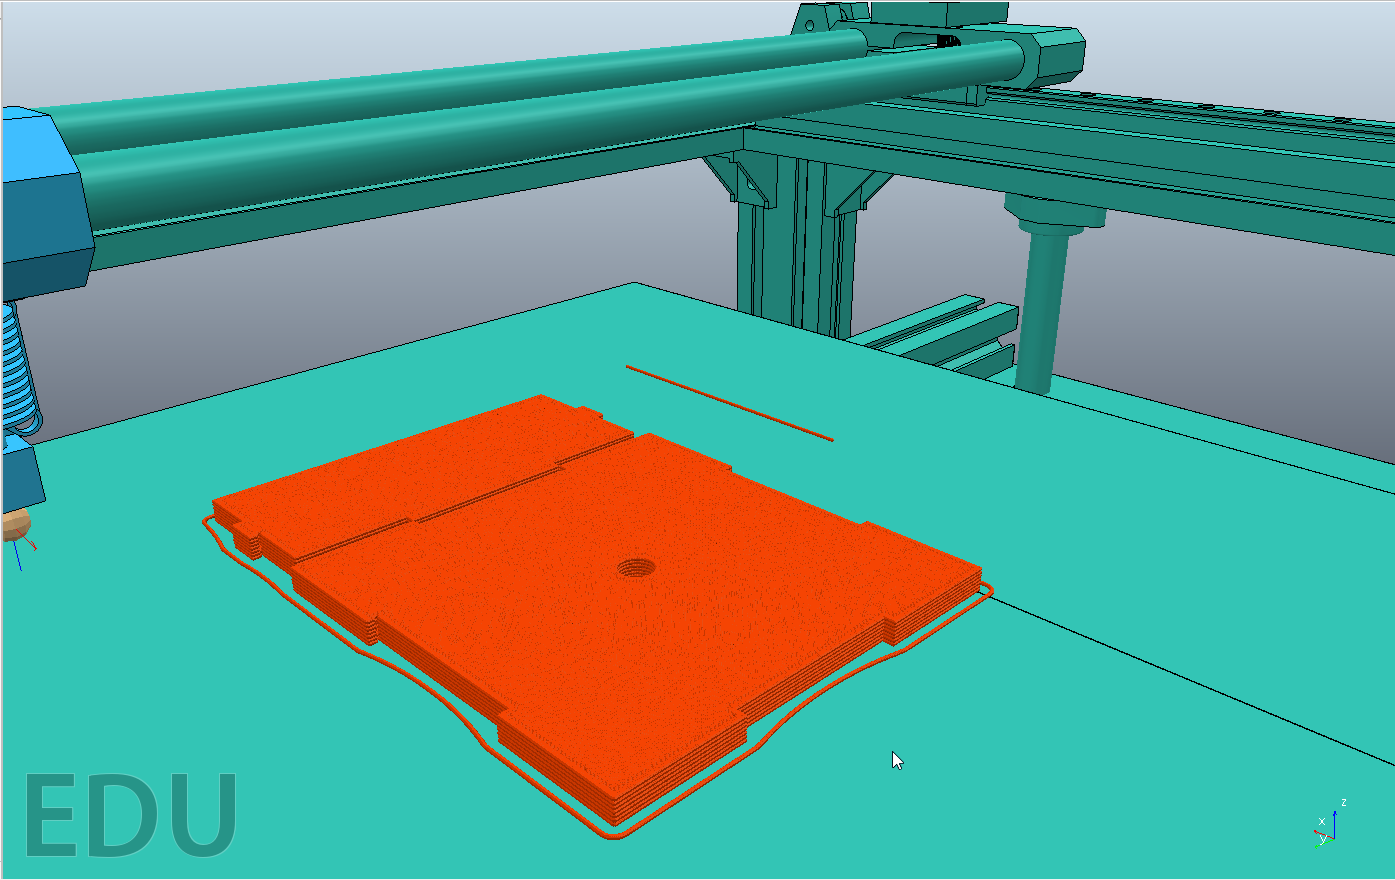
\includegraphics[width=8cm]{simulation}
\caption{\Large 模擬列印結果}\label{simulation}
\end{center}
\end{figure}

\newpage

